\documentclass[portrait,a0paper,fontscale=0.3085]{baposter}

\usepackage{calc}
\usepackage{graphicx}
\usepackage{amsmath}
\usepackage{amssymb}
\usepackage{relsize}
\usepackage{multirow}
\usepackage{rotating}
\usepackage{bm}
\usepackage{url}
\usepackage{graphicx}
\usepackage{multicol}
\usepackage{enumitem}
\usepackage[export]{adjustbox}% http://ctan.org/pkg/adjustbox

%\usepackage{times}
%\usepackage{helvet}
%\usepackage{bookman}
\usepackage{palatino}

\newcommand{\captionfont}{\footnotesize}

\graphicspath{{images/}{../images/}}
\usetikzlibrary{calc}

%%%%%%%%%%%%%%%%%%%%%%%%%%%%%%%%%%%%%%%%%%%%%%%%%%%%%%%%%%%%%%%%%%%%%%%%%%%%%%%%
%%%% Some math symbols used in the text
%%%%%%%%%%%%%%%%%%%%%%%%%%%%%%%%%%%%%%%%%%%%%%%%%%%%%%%%%%%%%%%%%%%%%%%%%%%%%%%%

%%%%%%%%%%%%%%%%%%%%%%%%%%%%%%%%%%%%%%%%%%%%%%%%%%%%%%%%%%%%%%%%%%%%%%%%%%%%%%%%
% Multicol Settings
%%%%%%%%%%%%%%%%%%%%%%%%%%%%%%%%%%%%%%%%%%%%%%%%%%%%%%%%%%%%%%%%%%%%%%%%%%%%%%%%
\setlength{\columnsep}{1.5em}
\setlength{\columnseprule}{0mm}

%%%%%%%%%%%%%%%%%%%%%%%%%%%%%%%%%%%%%%%%%%%%%%%%%%%%%%%%%%%%%%%%%%%%%%%%%%%%%%%%
% Save space in lists. Use this after the opening of the list
%%%%%%%%%%%%%%%%%%%%%%%%%%%%%%%%%%%%%%%%%%%%%%%%%%%%%%%%%%%%%%%%%%%%%%%%%%%%%%%%
\newcommand{\compresslist}{%
\setlength{\itemsep}{1pt}%
\setlength{\parskip}{0pt}%
\setlength{\parsep}{0pt}%
}

\begin{document}
\begin{poster}%
  % Poster Options
  {
  % Show grid to help with alignment
  grid=false,
  % Column spacing
  colspacing=1em,
  % Color style
  bgColorOne=white,
  bgColorTwo=white,
  borderColor=black,
  headerColorOne=red,
  headerColorTwo=red,
  headerFontColor=white,
  boxColorOne=white,
  % Format of textbox
  textborder=roundedleft,
  % Format of text header
  eyecatcher=true,
  headerborder=closed,
  headerheight=0.135\textheight,
%  textfont=\sc, An example of changing the text font
  headershape=roundedright,
  headershade=shadelr,
  headerfont=\Large\bf\textsc, %Sans Serif
  textfont={\setlength{\parindent}{1.5em}},
  boxshade=plain,
%  background=shade-tb,
  background=plain,
  linewidth=2pt
  }
  % Eye Catcher
  {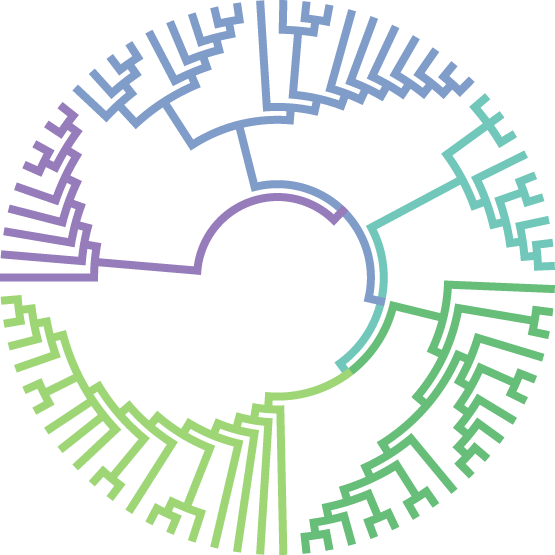
\includegraphics[height=7.0em]{images/rambaut_group_logo}} 
  % Title
  {\bf\textsc{Phylodynamics of Ebola in West Africa\linespread{0.25}\par}\vspace{0.25em}}
  % Authors
  {\textsc{Luiz Max de Carvalho$^{1,}$\footnote{{\small \texttt{lm.carvalho@ed.ac.uk} $^1$ Institute of Evolutionary Biology, University of Edinburgh, UK.}}\& Andrew Rambaut$^1$}\\}
  % University logo
  { 
\includegraphics[height=7.0em]{images/edi_logo}}
%%%%%%%%%%%%%%%%%%%%%%%%%%%%%%%%%%%%%%%%%%%%%%%%%%%%%%%%%%%%%%%%%%%%%%%%%%%%%%
\headerbox{Background}{name=problem,column=0,row=0}{
%%%%%%%%%%%%%%%%%%%%%%%%%%%%%%%%%%%%%%%%%%%%%%%%%%%%%%%%%%%%%%%%%%%%%%%%%%%%%%
\begin{itemize}[leftmargin=*]
 \subsubsection*{Mode and tempo of the epidemic}
 \item The 2013-2016 West African Ebola virus disease (EVD) epidemic was the largest in history;
 \item A massive international collaboration produced the most comprehensive data set for an acute virus to date (over 5\% sampling);
 \item Dudas et al. (2016) produced a rich data set with detailed information about viral movement in West Africa using $1610$ viral genomes;
 \item Our challenge is to combine different sources of information (epidemiological, genetic, climatic, etc) to trace the epidemic and explain its mode and \texit{tempo}.
 \item[\blacktriangleright] Which climatic and socio-economic factors predict outbreak sizes? 
 \subsubsection*{Association between a particular mutation and disease severity}
 \item There is experimental evidence that an A$\rightarrow$V mutation in the glycoprotein (GP) confers increased infectivity in human cells;
 \item[\blacktriangleright] Investigate the association between GP82-AV and disease severity using $236$ genomes for which clinical metadata was available;
  \end{itemize}
}
%%%%%%%%%%%%%%%%%%%%%%%%%%%%%%%%%%%%%%%%%%%%%%%%%%%%%%%%%%%%%%%%%%%%%%%%%%%%%%%%%
%%%%%%%%%%%%%%%%%%%%%%%%%%%%%%%%%%%%%%%%%%%%%%%%%%%%%%%%%%%%%%%%%%%%%%%%%%%%%%%%%
\headerbox{Results}{name=results,column=1,span=2,row=0}{
\includegraphics[scale=0.19,valign=c]{images/case-count_coefficients.png}\\
\textbf{Predictors of EVD outbreak sizes in West Africa}.
We show the predictors with Bayes factor (BF) larger than 3.
We find that low temperature seasonality and higher levels of rain increase the risk of larger outbreaks.
Similarly, urbanicity seems to play a role, with locations closer to urban centres being at higher risk.\\
\\
%%%%%%%%%%%%%%%%%%%%%%%%%%%%%%%%%%%%%%%%%%%%%%%%%%%%%%%%%%%%%%%%%%%%%%%%%%%%%%%%%
 \begin{tabular}{cc}
 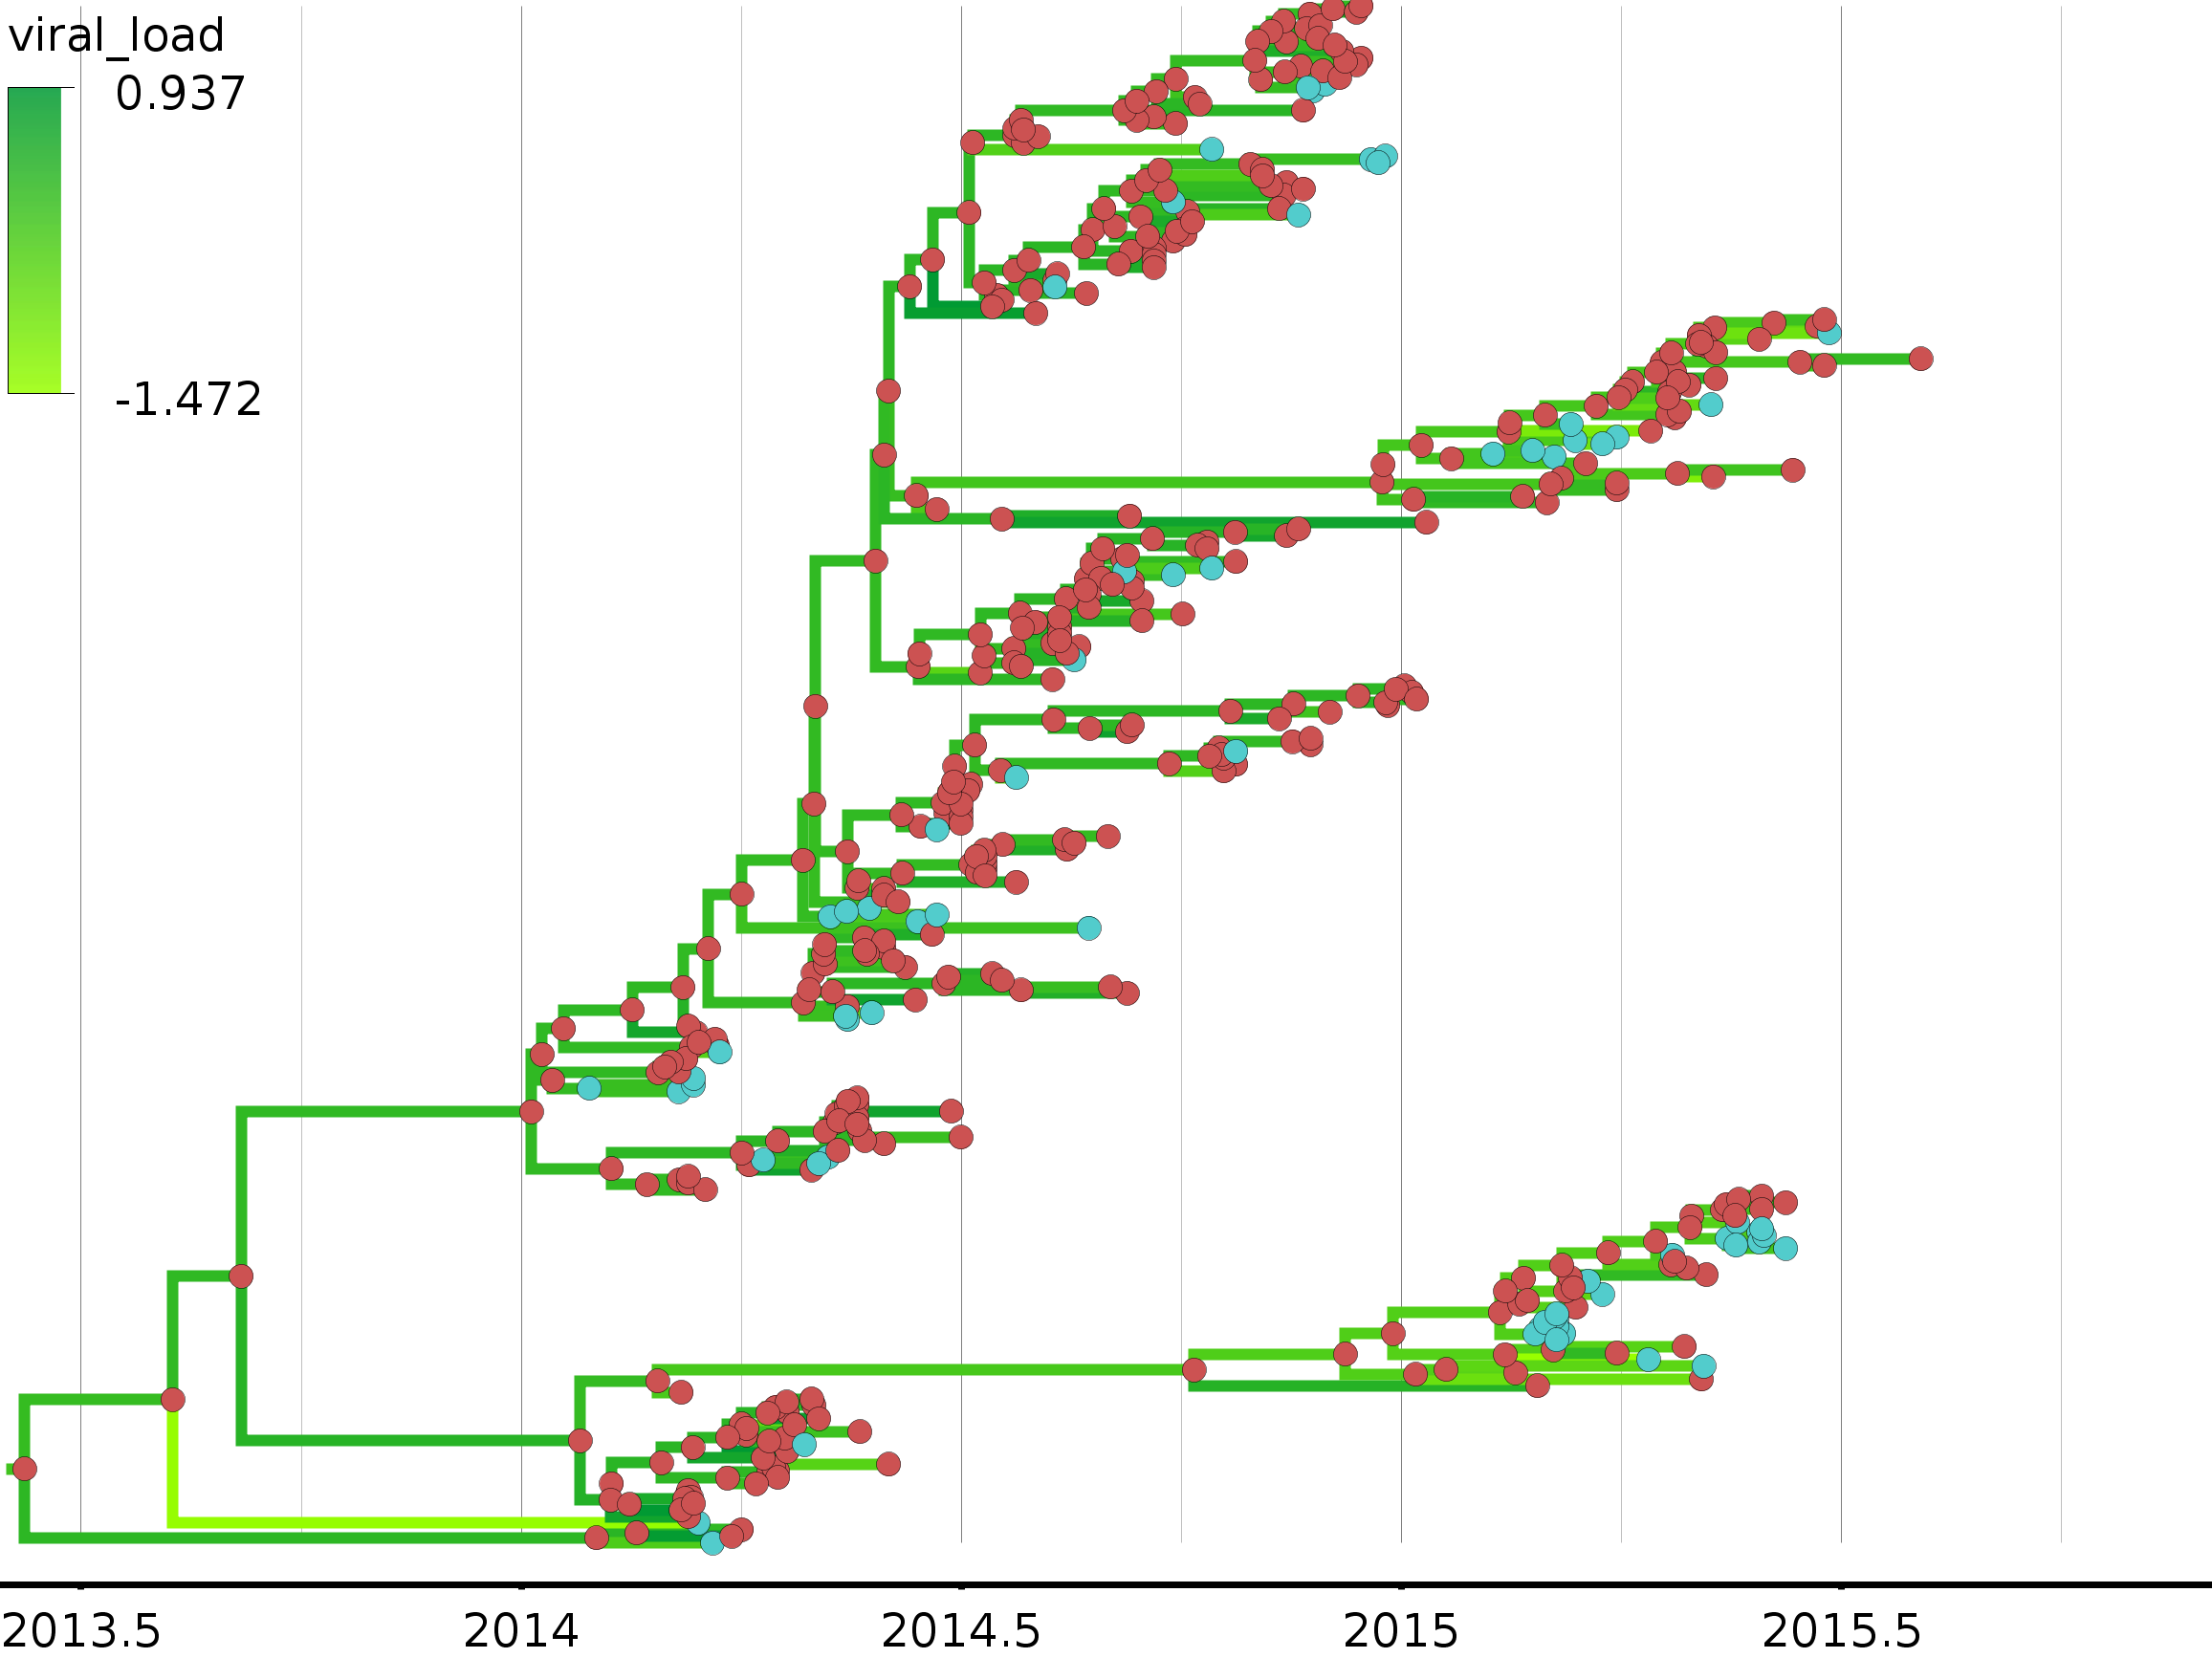
\includegraphics[scale=0.1,valign=c]{images/EVD_traits_tree.png} &
 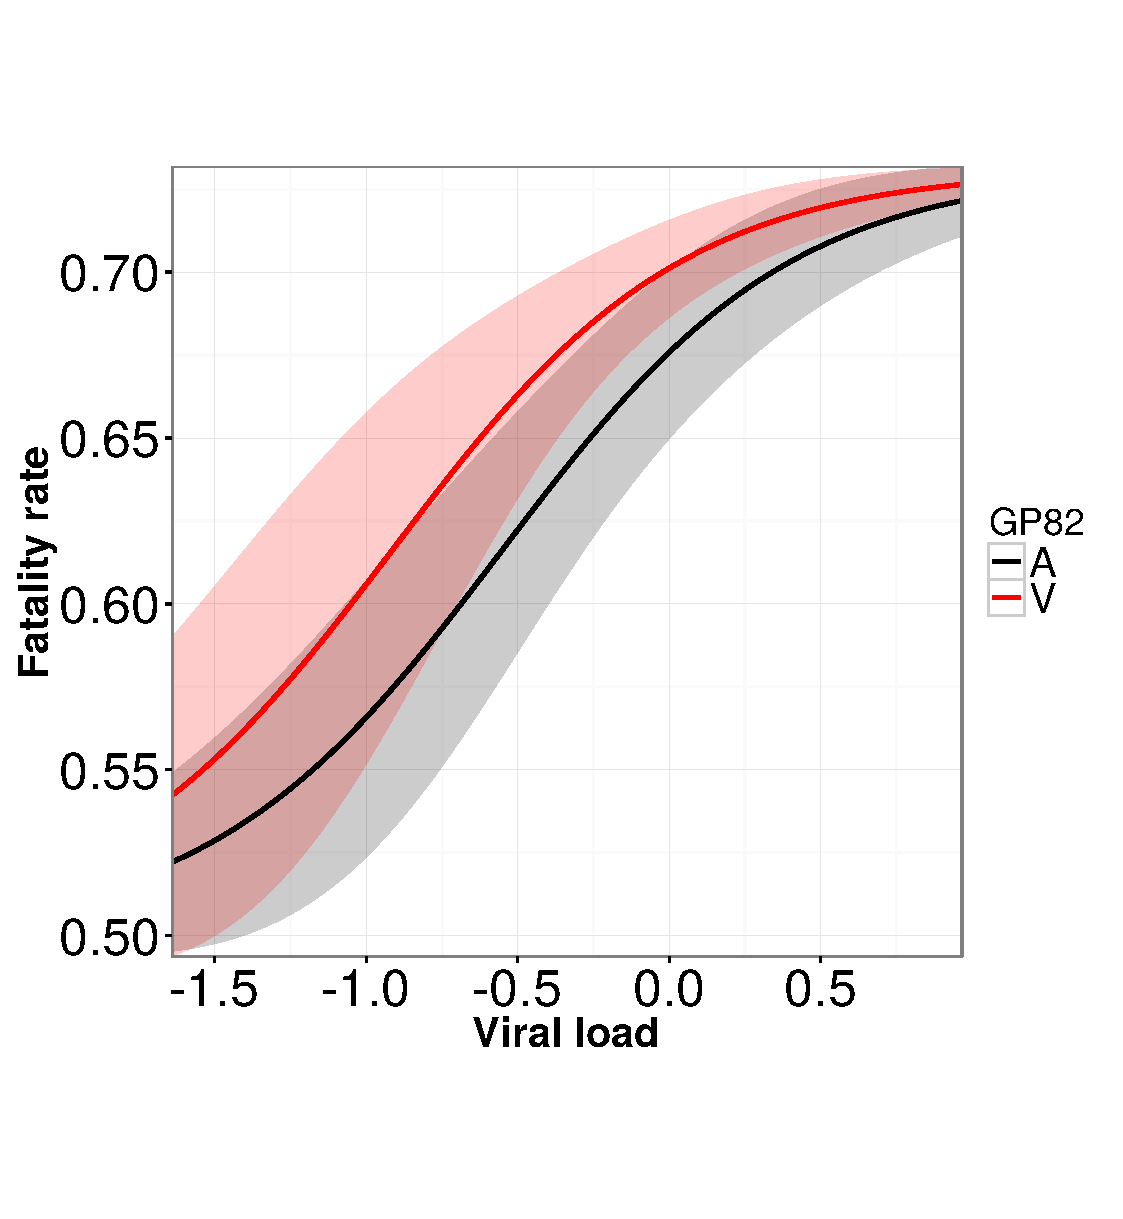
\includegraphics[scale=0.35,valign=c]{images/predicted_fatality_rates.pdf}
\end{tabular} \\
\\
\textbf{Association between the GP82-AV and disease severity.}
In the left panel we show a time-calibrated phylogeny with 236 sequences from patients whose outcome information was available.
Branches with lower viral loads (transformed $C(t)$) have higher probability of leading to surviving tips, suggesting some degree of heritability of infectivity.
The right panel shows the predicted fatality rates conditional on viral load for each genotype (wild type: \textbf{A}, mutant: \textbf{V}).
Notice that although fatality rates seem be higher for \textbf{V} the confidence bands overlap considerably, indicating substantial uncertainty.\\
\\
%%%%%%%%%%%%%%%%%%%%%%%%%%%%%%%%%%%%%%%%%%%%%%%%%%%%%%%%%%%%%%%%%%%%%%%%%%%%%%%%%% 
\begin{tabular}{ccc}
 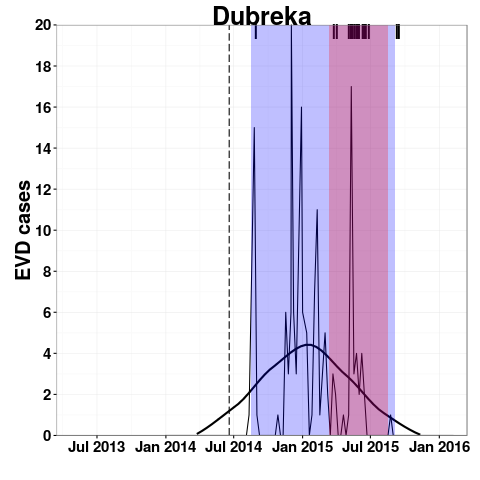
\includegraphics[scale=0.34,valign=c]{images/maxCases_Dubreka.png} &
 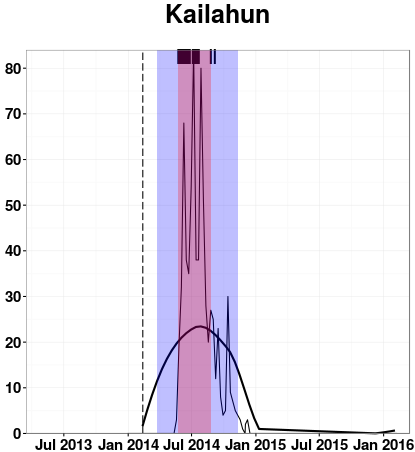
\includegraphics[scale=0.34,valign=c]{images/maxCases_Kailahun.png}&
 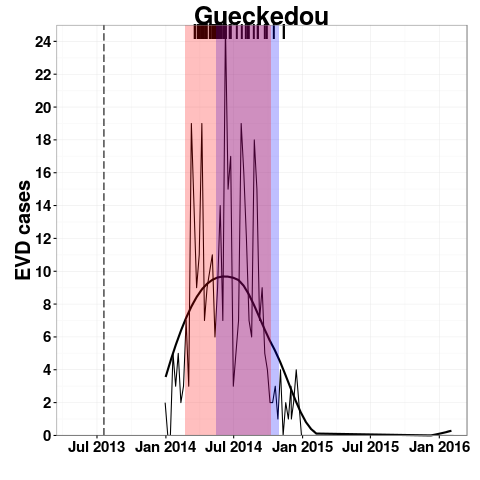
\includegraphics[scale=0.34,valign=c]{images/maxCases_Gueckedou.png}
\end{tabular}\\

\textbf{Combining epidemiological and genetic data}.
Here we overlay case notifications data with inferred introductions to gain insight into the dynamics of EVD the epidemic.
Dashed vertical line marks the earliest introduction in the posterior.
Shaded areas show the 95\% credibility interval for introductions (blue) and exports (red).
Rugplots show dates of sampling of the sequences in that location.
\section*{Conclusions}
\begin{itemize}
 \item Both climatic and social economic factors predict outbreak sizes.
 We have employed this approach to help explain why some regions did not experience cases despite being in close proximity with affected areas.
 \item The A$\rightarrow$V mutation in the EBOV glycoprotein is weakly associated with higher fatality rates;
 \item By combining epidemiological information and viral movement inferred from sequenced genomes one can gain insight into the dynamics of Ebola in West Africa.
 Our challenge now is to integrate all of this information in a coherent statistical model.
\end{itemize}

Funding: I thank the School of Biological Sciences for topping up my stipend.
}
% %%%%%%%%%%%%%%%%%%%%%%%%%%%%%%%%%%%%%%%%%%%%%%%%%%%%%%%%%%%%%%%%%%%%%%%%%%%%%%%%%
% \headerbox{Conclusions}{name=conclusions,column=1,span=2,below=results}{
% %%%%%%%%%%%%%%%%%%%%%%%%%%%%%%%%%%%%%%%%%%%%%%%%%%%%%%%%%%%%%%%%%%%%%%%%%%%%%%%%%
% \begin{itemize}
%  \item Both climatic and social economic factors predict outbreak sizes.
%  We have employed this approach to help explain why some regions did not experience cases despite being in close proximity with affected areas.
%  \item The A$\rightarrow$V mutation in the EBOV glycoprotein is weakly associated with higher fatality rates;
%  \item By combining epidemiological information and viral movement inferred from sequenced genomes one can gain insight into the dynamics of Ebola in West Africa.
%  Our challenge now is to integrate all of this information in a coherent statistical model.
% \end{itemize}
% 
% Funding: I thank the School of Biological Sciences for topping up my stipend.
% }
%%%%%%%%%%%%%%%%%%%%%%%%%%%%%%%%%%%%%%%%%%%%%%%%%%%%%%%%%%%%%%%%%%%%%%%%%%%%%%
\headerbox{Methods}{name=method,column=0,below=problem}{
%%%%%%%%%%%%%%%%%%%%%%%%%%%%%%%%%%%%%%%%%%%%%%%%%%%%%%%%%%%%%%%%%%%%%%%%%%%%%%
We take a Bayesian approach and estimate time-calibrated phylogenies with \textbf{BEAST}.
\begin{itemize}[leftmargin=*]
 \item[$\oint$] Case counts ($\mathbf{Y}$) along climatic and socio-economic covariates ($\mathbf{X}$) for $56$ locations $\rightarrow$ negative binomial GLM + SSVS:
\begin{align*}
 Y_i & \sim \text{NegBin}(p_i, r) \\
 p_i & = \frac{r}{(r + \lambda_i)}  \\ 
\log(\lambda_i) &= \alpha + \beta_{1}\delta_{1} x_{i1} + \ldots + \beta_{P}\delta_{P} x_{iP} 
\end{align*}
This approach has the advantage of allowing for the calculation of Bayes factors (BF) analytically.
Let (prior) $w_0$ the probability that no predictors are included. 
Then the Bayes factor for predictor $x_j$ is
\begin{equation*}
 \text{BF}(x_j) = \frac{\hat{\delta_j}w_0^{1/P}}{(1-\hat{\delta_j})(1 - w_0^{1/P})}
\end{equation*}
where $P$ is the number of predictors.
%%%%%%%%%%%%%%%%%%%%%%%%%%%%%%%%%%%%%%%%%%%%%%%%%
 \item[$\oint$] We had viral load ($C(t)$ values) and outcome (death/survival) information for $236$ patients $\rightarrow$ binomial GLM;
%%%%%%%%%%%%%%%%%%%%%%%%%%%%%%%%%%%%%%%%%%%%%%%%%
 \item[$\oint$] Constructing outbreak clusters: every time a location receives a viral introduction that leads to $>$20 sampled cases, split the series before and after the introduction.
\end{itemize}
}
\end{poster}
\end{document}